\documentclass[]{standalone}
\usepackage{mathptmx}
\renewcommand{\familydefault}{\rmdefault}
\usepackage[T1]{fontenc}
\usepackage[latin9]{inputenc}
\usepackage{siunitx}
\usepackage{array}
\usepackage{amsmath}
\usepackage{ifthen}
\usepackage{pgfplots}
\usepackage{pgfmath}
\pgfplotsset{compat=1.14}
\usepackage{titling, graphicx}
\usepackage{tikz}
\usepackage{upgreek}
\usepackage{amsmath,amsthm}
\usepackage{strtikz}
\usetikzlibrary{shapes,arrows.meta,intersections,graphs,graphs.standard,math,fit}
\usetikzlibrary{calc,intersections,through,backgrounds}
\usetikzlibrary{decorations.pathmorphing, decorations.markings,decorations.pathreplacing}


\begin{document}
\begin{tikzpicture}
\sdofsys[startx = 0cm, starty = 0cm,
  support width = 4.0cm,
  support height = 1.5cm,
  vertical support line thickness = 1pt,
  horizontal support line thickness = 1pt,
  vertical support shade thickness = 0.3cm,
  horizontal support shade thickness = 0.3cm,    
  mass line thickness = 1pt,
  mass height = 1cm,
  mass width = 1.5cm,
  massx = 1.5cm,
  mass text = $m$,
  spring and damper line thickness = 0.5pt,
  spring location ratio = 0.25,
  spring ratio = 0.15,
  spring zigzag amplitude = 0.1cm,
  spring zigzag segment length = 0.2cm,
  spring text = $k$,
  spring text side = above,
  damper width ratio = 0.15,
  damper height ratio = 0.3,
  damper piston size ratio = 0.7,
  damper piston position ratio = 0.5,
  damper text = $c$,
  damper text side = 2,
  wheel line thickness = 1pt,
  wheel radius = 0.15cm,
  wheel location ratio = 0.25,
  wheel size ratio = 1,
  disp line location ratio = 0.5,
  disp line = 0.25cm,
  disp arrow = 0.5cm,
  disp text = $x(t)$,
  disp line thickness = 0.5pt,
  forcex location ratio = 1.0,
  forcey location ratio = 0.5,  
  force length = 1cm,
  force line thickness = 0.5pt,
  force text = $f(t)$,
  display displacement = 1,
  display force = 1]
\end{tikzpicture}
\end{document}